\let\negmedspace\undefined
\let\negthickspace\undefined
\documentclass[journal]{IEEEtran}
\usepackage[a5paper, margin=10mm, onecolumn]{geometry}
%\usepackage{lmodern} % Ensure lmodern is loaded for pdflatex
\usepackage{tfrupee} % Include tfrupee package

\setlength{\headheight}{1cm} % Set the height of the header box
\setlength{\headsep}{0mm}     % Set the distance between the header box and the top of the text

\usepackage{gvv-book}
\usepackage{gvv}
\usepackage{cite}
\usepackage{titling}
\usepackage{amsmath,amssymb,amsfonts,amsthm}
\usepackage{algorithmic}
\usepackage{graphicx}
\usepackage{textcomp}
\usepackage{xcolor}
\usepackage{txfonts}
\usepackage{listings}
\usepackage{enumitem}
\usepackage{mathtools}
\usepackage{gensymb}
\usepackage{comment}
\usepackage[breaklinks=true]{hyperref}
\usepackage{tkz-euclide} 
\usepackage{listings}
% \usepackage{gvv}                                        
\def\inputGnumericTable{}                                 
\usepackage[latin1]{inputenc}                                
\usepackage{color}                                            
\usepackage{array}                                            
\usepackage{longtable}                                       
\usepackage{calc}                                             
\usepackage{multirow}                                         
\usepackage{hhline}                                           
\usepackage{ifthen}                                           
\usepackage{lscape}
\begin{document}

\bibliographystyle{IEEEtran}
\vspace{3cm}

\title{DETT}
\author{EE24BTECH11010 - BALAJI B}
% \maketitle
% \newpage
% \bigskip
{\let\newpage\relax\maketitle}

\renewcommand{\thefigure}{\theenumi}
\renewcommand{\thetable}{\theenumi}
\setlength{\intextsep}{10pt} % Space between text and floats


\numberwithin{equation}{enumi}
\numberwithin{figure}{enumi}
\renewcommand{\thetable}{\theenumi}

\section{Introduction}
In this report, we focus on solving the first-order linear differential equation
\begin{align}
    L \frac{di}{dt} + Ri = v(t)
\end{align}
where $L$ and $R$ are constants representing inductance and resistance, respectively, and $v(t)$ is an applied voltage. Specifically, we consider $v(t)$ as a square wave, a commonly used signal in electronic circuits and signal processing. \\ \\ 
To solve this equation, we employ the Fast Fourier Transform (FFT), a powerful tool that converts differential equations into algebraic equations in the frequency domain, significantly reducing computational complexity. However, applying FFT directly to sampled data introduces numerical challenges, particularly aliasing and resolution errors. \\ \\ 
To address these issues, we implement Nyquist sampling, which ensures that our numerical solution retains accuracy and prevents distortions caused by insufficient sampling rates. By comparing the results before and after applying Nyquist sampling, we demonstrate its critical role in improving computational accuracy.
\section{Mathematical Formulation}
The given differential equation governing the system is:
\begin{align}
    L \frac{di}{dt} + Ri = v(t)
\end{align}
where:
\begin{itemize}
    \item $i(t)$ is the current as a function of time,
    \item $L$ is the inductance (in Henrys),
    \item $R$ is the resistance (in Ohms),
    \item $v(t)$ is the applied voltage, which is chosen to be a square wave.
\end{itemize}
\subsection{Fourier Transform Approach}
To solve this equation using the Fast Fourier Transform (FFT), we take the Fourier transform of both sides. The Fourier transform of a time-domain function $f(t)$ is defined as:
\begin{align}
    F(\omega) = \int_{-\infty}^{\infty} f(t) e^{-j\omega t} dt
\end{align}
Applying this to the given differential equation, we use the property that the Fourier transform of a derivative is given by:
\begin{align}
    \mathcal{F} \left( \frac{df}{dt} \right) = j\omega F(\omega)
\end{align}
Taking the Fourier transform of both sides:
\begin{align}
    L (j\omega I(\omega)) + R I(\omega) = V(\omega)
\end{align}
Rearranging for $I(\omega)$:
\begin{align}
    I(\omega) = \frac{V(\omega)}{R + j\omega L}
\end{align}
To obtain $i(t)$ in the time domain, we take the inverse Fourier transform:
\begin{align}
    i(t) = \mathcal{F}^{-1} \left( I(\omega) \right) = \mathcal{F}^{-1} \left( \frac{V(\omega)}{R + j\omega L} \right)
\end{align}
The inverse Fourier transform is computed numerically using the Inverse Fast Fourier Transform (IFFT) in practical implementations. This step allows us to reconstruct the time-domain current response from the frequency-domain solution.
\section{Solution Using FFT}
In this section, we numerically solve the differential equation
\begin{align}
    L \frac{di}{dt} + Ri = v(t)
\end{align}
using the Fast Fourier Transform (FFT). The FFT is used to transform the equation into the frequency domain, solve for $I(\omega)$, and then apply the Inverse Fast Fourier Transform (IFFT) to obtain $i(t)$ in the time domain.
\subsection{ Discretization of the Equation}
Since the FFT operates on discrete signals, we first sample the input voltage $v(t)$ at discrete time intervals:
\begin{align}
    t_k = k\Delta t, \quad k = 0, 1, 2,\dots, N-1
\end{align}
where $N$ is the number of samples, and $\Delta t$ is the sampling period. The sampled voltage is then stored as a sequence:
\begin{align}
    v[k] = v(t_k)
\end{align}
Applying the FFT to this discrete signal, we obtain its frequency-domain representation:
\begin{align}
    V[\omega] = \text{FFT}(v[k])
\end{align}
Similarly, the current $i(t)$ is represented as a sequence $i[k]$, whose frequency-domain representation is:
\begin{align}
    I[\omega] = \text{FFT}(i[k])
\end{align}
From the Fourier Transform solution derived in from previous section, we solve for $I[\omega]$ as:
\begin{align}
    I[\omega] = \frac{V[\omega]}{R + j\omega L}
\end{align}
where $\omega$ is the discrete frequency vector corresponding to the FFT output.
\subsection{Applying the Inverse FFT}
Once $I[\omega]$ is computed, we use the Inverse FFT (IFFT) to obtain the current in the time domain:
\begin{align}
    i[k] = \text{IFFT}(I[\omega])
\end{align}
This gives the numerical solution for $i(t)$, which represents the system's response to the square wave input.
\subsection{Numerical Considerations and Challenges
}
While using FFT provides an efficient solution, certain challenges must be addressed:
\begin{enumerate}
    \item \textbf{Aliasing}: If the sampling rate is too low, high-frequency components can be misrepresented.
    \item \textbf{Resolution Limitations}: The accuracy of the computed $i(t)$ depends on the number of samples $N$ and the choice of $\Delta t$.
    \item \textbf{Spectral Leakage}: Since a square wave consists of harmonics, improper windowing can distort the frequency spectrum.
\end{enumerate}
These issues will be mitigated using Nyquist sampling in the next section.
\subsection{Steady-State Nature of the FFT Solution}
The Fourier Transform approach provides a solution to the RL circuit equation in the \textbf{frequency domain}. However, it is important to note that this method inherently \textbf{excludes the transient response} of the circuit and only captures the \textbf{steady-state behavior}. \\ \\ 
\textbf{Why Does FFT Capture Only the Steady-State Response?}
\begin{enumerate}
    \item Fourier Transform Assumes a Periodic Input
    \begin{itemize}
        \item The FFT method works under the assumption that the input voltage signal $v(t)$ is periodic and extends infinitely in both directions.
        \item This assumption removes the initial transient effects that would naturally occur in a real RL circuit when the square wave is first applied.
    \end{itemize}
    \item Lack of Initial Condition Handling
    \begin{itemize}
        \item The time-domain solution of a first-order RL circuit typically consists of a transient term (exponential decay) and a steady-state term.
        \item he Fourier domain approach only considers the frequency response of the system and does not include any \textbf{initial condition information} (e.g., initial inductor current).
    \end{itemize}
    \item Inverse FFT Returns a Time-Periodic Solution
    \begin{itemize}
        \item Since the input square wave is treated as a periodic function, the inverse FFT retrieves a steady-state solution that assumes the circuit has already settled into a periodic response.

    \end{itemize}
\end{enumerate}

\section{ Nyquist Sampling and Its Significance}
In the previous section, we computed the current response $i(t)$ using the Fast Fourier Transform (FFT). However, when solving differential equations numerically, the accuracy of the solution depends heavily on how the input signal is sampled. In this section, we discuss the Nyquist sampling theorem and demonstrate its role in improving computational accuracy.
\subsection{Nyquist Sampling Theorem}
The Nyquist theorem states that a continuous signal can be accurately reconstructed from its discrete samples if the sampling rate $f_s$ satisfies:
\begin{align}
    f_s \geq 2 f_{\max}
\end{align}
where $f_{\max}$ is the highest frequency component present in the signal. If the sampling rate is too low (i.e., $f_s < 2 f_{\max})$, aliasing occurs, causing high-frequency components to be misrepresented as lower frequencies, distorting the signal.
\subsection{Square Wave with Duty Factor}
A square wave with a duty cycle D is defined as:
\begin{align}
    v(t) =
\begin{cases}
V_{\max}, & 0 \leq t < D T \\
V_{\min}, & D T \leq t < T
\end{cases}
\end{align}
where:
\begin{itemize}
    \item $T = 1/f_0$ is the period of the wave,
    \item D is the duty cycle (e.g., $50$ \% for a symmetric square wave, $<50$ \% for a narrow pulse, $>50$ \% for a wide pulse).
\end{itemize}
Unlike a $50$ \% duty cycle square wave, which contains only odd harmonics, a general duty cycle introduces additional frequency components, including even harmonics. The harmonic content depends on $D$, and capturing it correctly requires sufficient sampling resolution.
\subsection{Effect of Nyquist Sampling on the Computed Current Response}
By applying Nyquist sampling, we mitigate aliasing and improve the numerical accuracy of $i(t)$. Key improvements include:
\begin{enumerate}
    \item \textbf{Reduction of Aliasing Errors}: Ensuring that the FFT does not misinterpret high-frequency content.
    \item \textbf{Preservation of Pulse Shape}: Since the duty cycle affects the waveform's spectral content, sufficient sampling ensures that narrow or wide pulses are accurately represented.
    \item 	\textbf{Better Frequency Resolution}: The FFT correctly captures the harmonic structure dictated by the duty cycle.
    \item \textbf{Convergence of Output with Sufficient Sampling}: After a certain sampling rate, further increasing $f_s$ does not significantly alter the output wave.
\end{enumerate}
\subsection{Choosing an Optimal Sampling Rate}
A key observation is that once the sampling rate exceeds a certain threshold, \textbf{increasing it further does not significantly change the output current waveform}. This occurs because:
\begin{itemize}
    \item The essential harmonic components have already been captured.
    \item The circuit itself acts as a low-pass filter, naturally attenuating higher harmonics.
    \item Additional high-frequency components beyond a certain range contribute negligibly to the shape of $i(t)$.
\end{itemize}

 \textbf{Experimental Observation}
 To illustrate this, we compute i(t) for multiple sampling rates: \\ 
     \begin{center}
          Below Nyquist Rate $(f_s < 2 f_{\max})$: 
     \end{center}
    \captionsetup{type=figure}
    \centering
    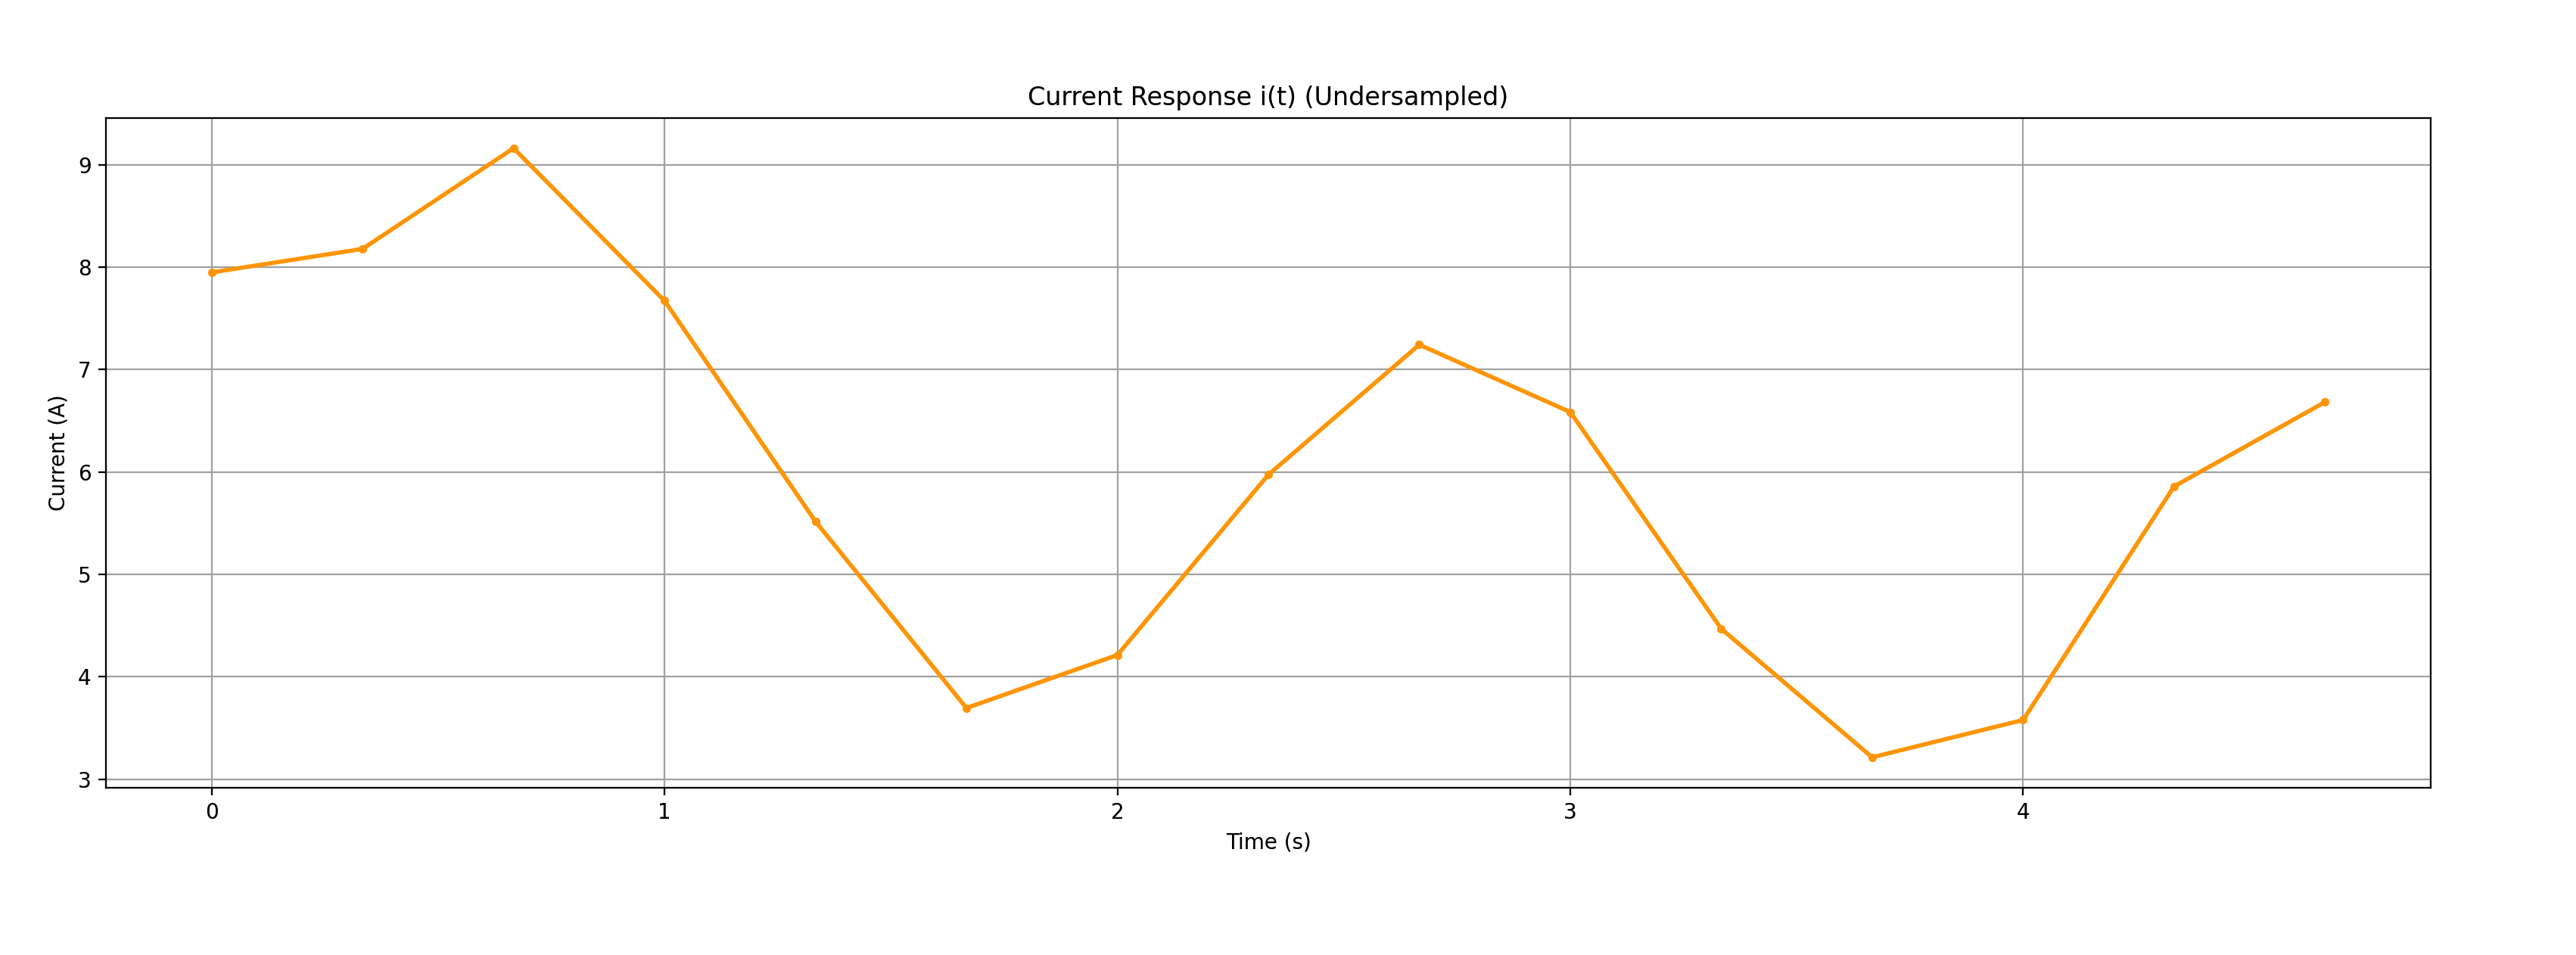
\includegraphics[width=0.6\textwidth]{Nyquist_samples/0_75f_ny}
    \caption{The current response for  $f_s < f_{ny}$   i.e, $(0.75*f_{ny})$}
    \label{fig:example}
      \begin{itemize}
          \item The square wave appears distorted, with missing transitions or incorrect duty cycle representation.
          \item The computed $i(t)$ is inaccurate due to aliasing.
          \item The FFT spectrum shows incorrect frequency content.
      \end{itemize}
    \begin{center}  
      Slightly Above Nyquist Rate: 
    \end{center}
      
      \captionsetup{type=figure}
    \centering
    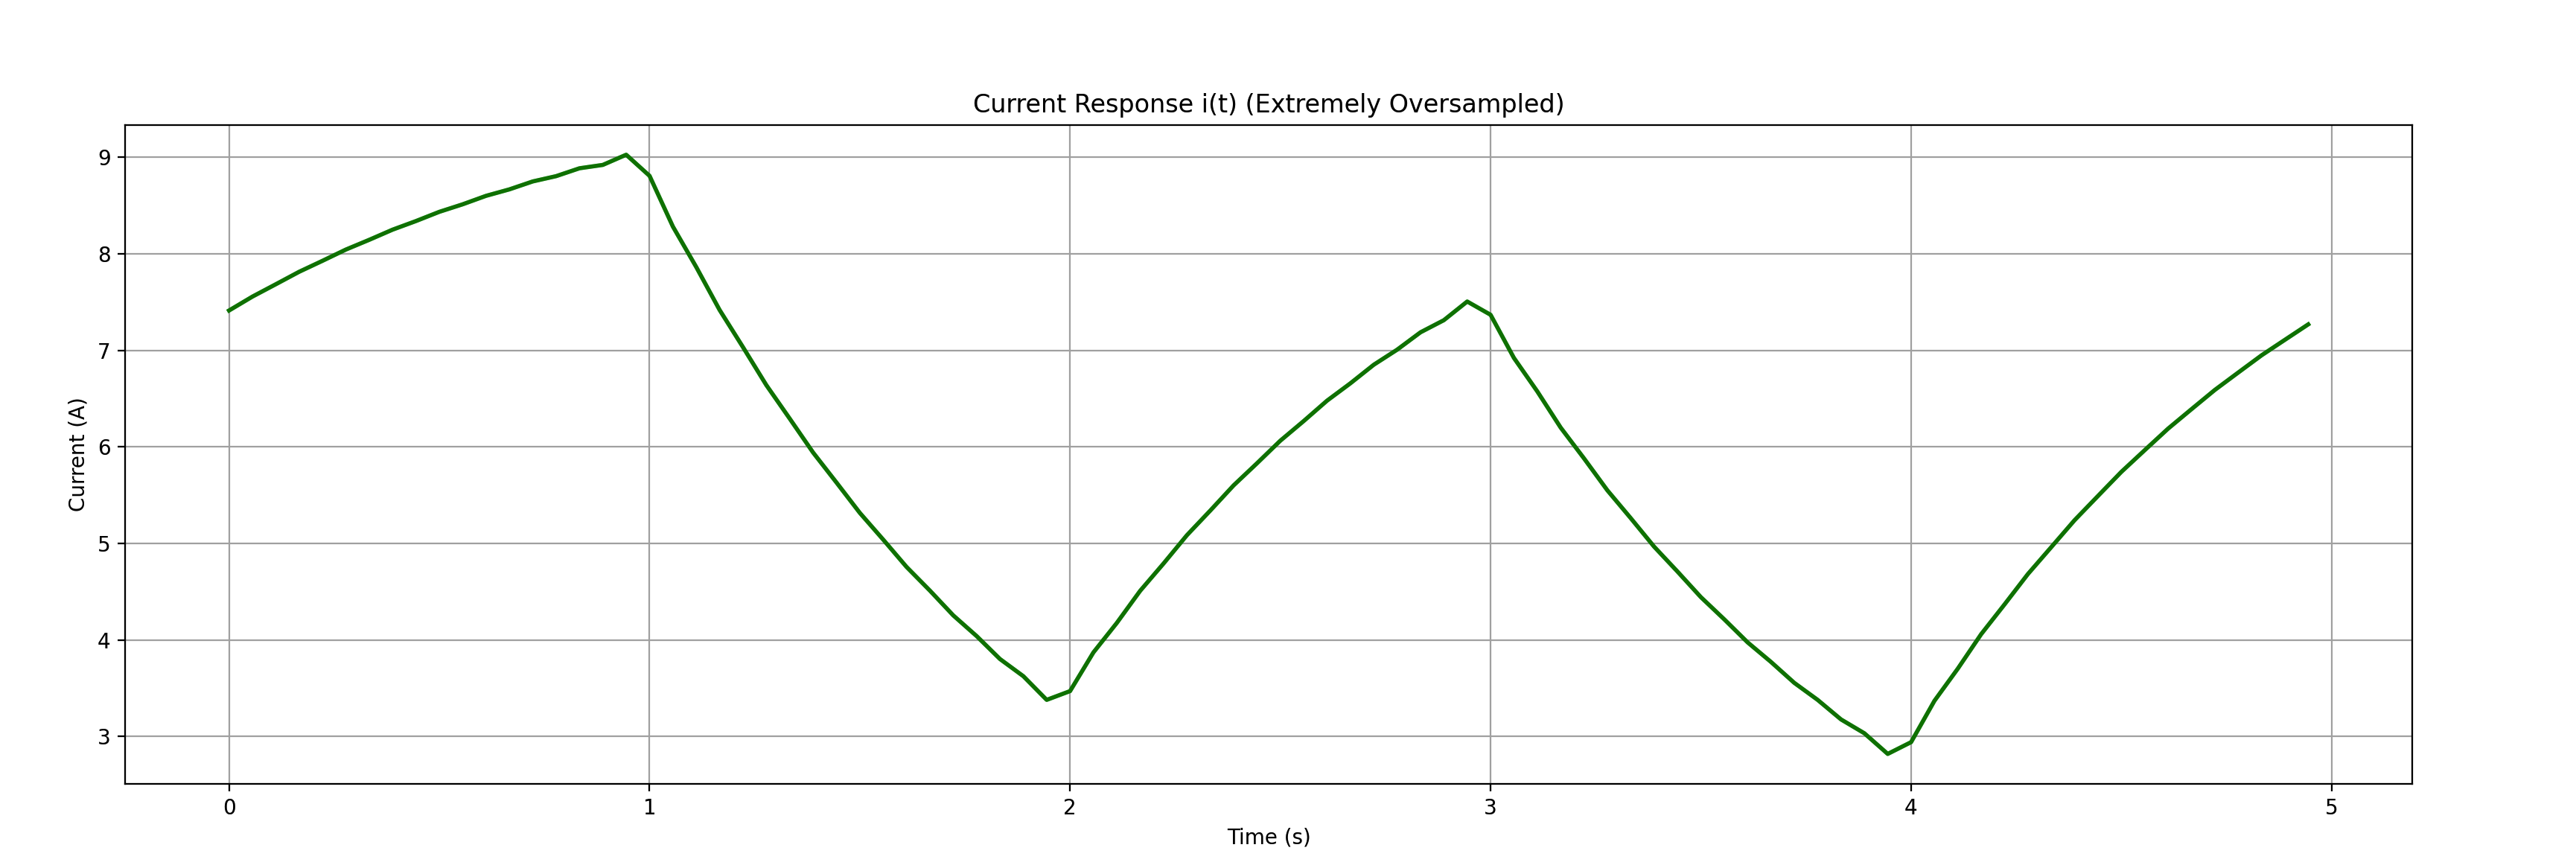
\includegraphics[width=0.6\textwidth]{Nyquist_samples/4_f_ny}
    \caption{The current response for  $f_s > f_{ny}$   i.e, $(4f_{ny})$}
    \label{fig:example}
    \begin{itemize}
        \item The waveform is well-preserved, and the current response $i(t)$ matches expected results.
        \item Harmonic content is properly captured.
    \end{itemize}
    \begin{center} 
     Very High Sampling Rate $(f_s \gg 2 f_{\max}):$
    \end{center}
     \captionsetup{type=figure}
    \centering
    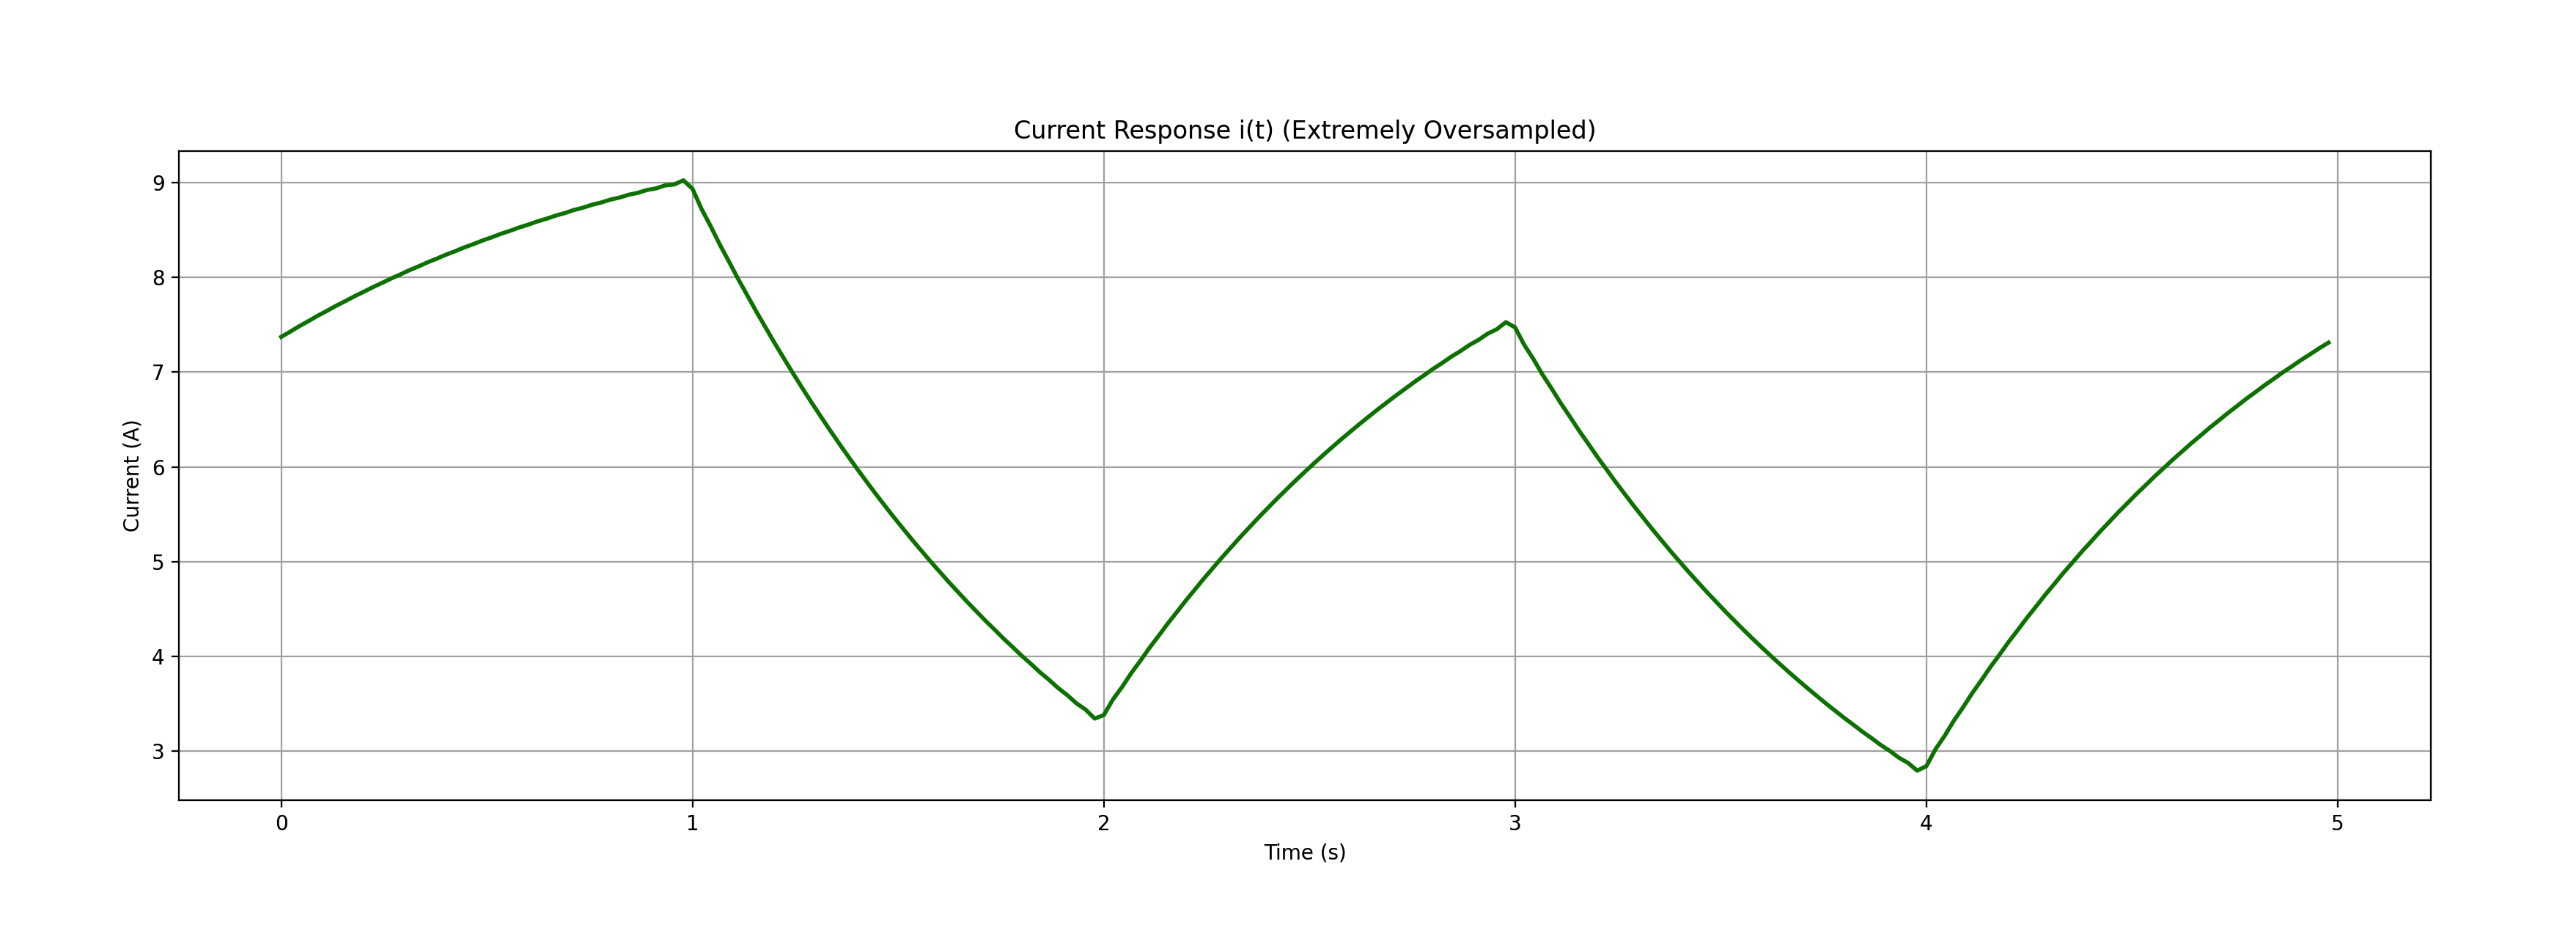
\includegraphics[width=0.6\textwidth]{Nyquist_samples/10_f_ny}
    \caption{The current response for  $f_s \gg f_{ny}$   i.e, $(10 f_{ny})$}
    \label{fig:example}
    \begin{itemize}
        \item 	No significant change in the output waveform is observed.
        \item Computation time increases, but results remain nearly the same.
    \end{itemize}
    
\subsection{Conclusion: Selecting an Efficient Sampling Rate}
      From these observations, we conclude:
    \begin{itemize}
        \item A sampling rate \textbf{just above} the Nyquist limit is sufficient to capture the waveform accurately.
        \item Further increasing $f_s$ \textbf{beyond a certain point does not change $i(t)$ significantly}, making higher sampling rates unnecessary.
        \item he choice of $f_s$ should balance \textbf{accuracy and computational efficiency}.
    \end{itemize}
 \section{Computational Implementation and Results}
 In this section, we present the numerical implementation of the RL circuit response to a square wave voltage input. The computational approach involves:
 \begin{enumerate}
     \item Generating a \textbf{square wave} with a specified duty cycle.
     \item Computing the \textbf{current response} using the \textbf{Fast Fourier Transform (FFT).}
     \item Applying \textbf{Nyquist sampling} to analyze its effect on accuracy.
     \item \textbf{Visualizing} the results with adjustable parameters
 \end{enumerate}
 \subsection{Numerical Implementation}
 The implementation is done using \textbf{Python} with \textbf{NumPy, SciPy}, and \textbf{Matplotlib}. The key components of the code are:
 \begin{itemize}
     \item \textbf{Square Wave Generation}: The input voltage $v(t)$ is generated directly using a periodic function rather than Fourier synthesis. The duty cycle can be adjusted dynamically.
     \item \textbf{Fourier Transform Approach}: FFT is applied to transform $v(t)$ into the frequency domain, where the circuit's response is computed.
     \item \textbf{Inverse FFT for i(t)}: The computed current spectrum $I(\omega)$ is transformed back into the time domain using \textbf{IFFT.}
     \item \textbf{Nyquist Sampling}: The effect of different sampling rates on $v(t)$ and $i(t)$ is studied.
 \end{itemize}
 \subsubsection{Solving for $i(t)$ in the Frequency Domain}
Using FFT, the circuit's response is computed by solving:
\begin{align}
    I(\omega) = H(\omega) V(\omega)
\end{align}
where the transfer function is:
\begin{align}
    H(\omega) = \frac{1}{R + j\omega L}
\end{align}
The inverse FFT then retrieves $i(t)$ in the time domain.
\subsection{Results and Discussion}
\subsubsection{Square Wave Representation}
\begin{itemize}
    \item \textbf{High-Resolution Input Signal}: The first plot shows the square wave sampled at a high resolution to approximate a continuous-time signal.
    \item \textbf{Nyquist-Sampled Square Wave}: The second plot shows the same signal sampled at the Nyquist rate, which captures the key frequency components without excessive data points.
\end{itemize}
\subsubsection{Current Response Analysis}
\begin{itemize}
    \item \textbf{High-Resolution Current Response $i(t)$}: The third plot presents the current waveform when using a very fine sampling rate.
    \item \textbf{Nyquist-Sampled Current Response}: The final plot shows the current response when sampling at the Nyquist rate.
\end{itemize}
\subsubsection{Key Observations}
\begin{enumerate}
    \item \textbf{Nyquist Sampling Preserves Accuracy}: The sampled square wave retains its fundamental characteristics without significant loss of information.
    \item \textbf{Smoothing Effect of the Circuit}: The RL circuit naturally filters higher harmonics, making the response smoother compared to the input square wave.
    \item \textbf{After a Certain Sampling Rate, $i(t)$ Converges}: Increasing the sampling rate beyond a certain point does not significantly change the computed response.
\end{enumerate}
\subsection{Interactive Parameter Tuning}
The implementation includes \textbf{interactive sliders} for adjusting:
\begin{itemize}
    \item Resistance $R$
    \item Inductance $ L$
    \item Square wave period $T$
    \item Number of harmonics
    \item Duty cycle
    \item Amplitude
    \item Simulation time
\end{itemize}
These controls allow for real-time observation of how circuit parameters influence i(t).

\subsection{Visualization of Results}
\textbf{The Plot of the current response through FFT}
\begin{figure}[H]
    \centering
    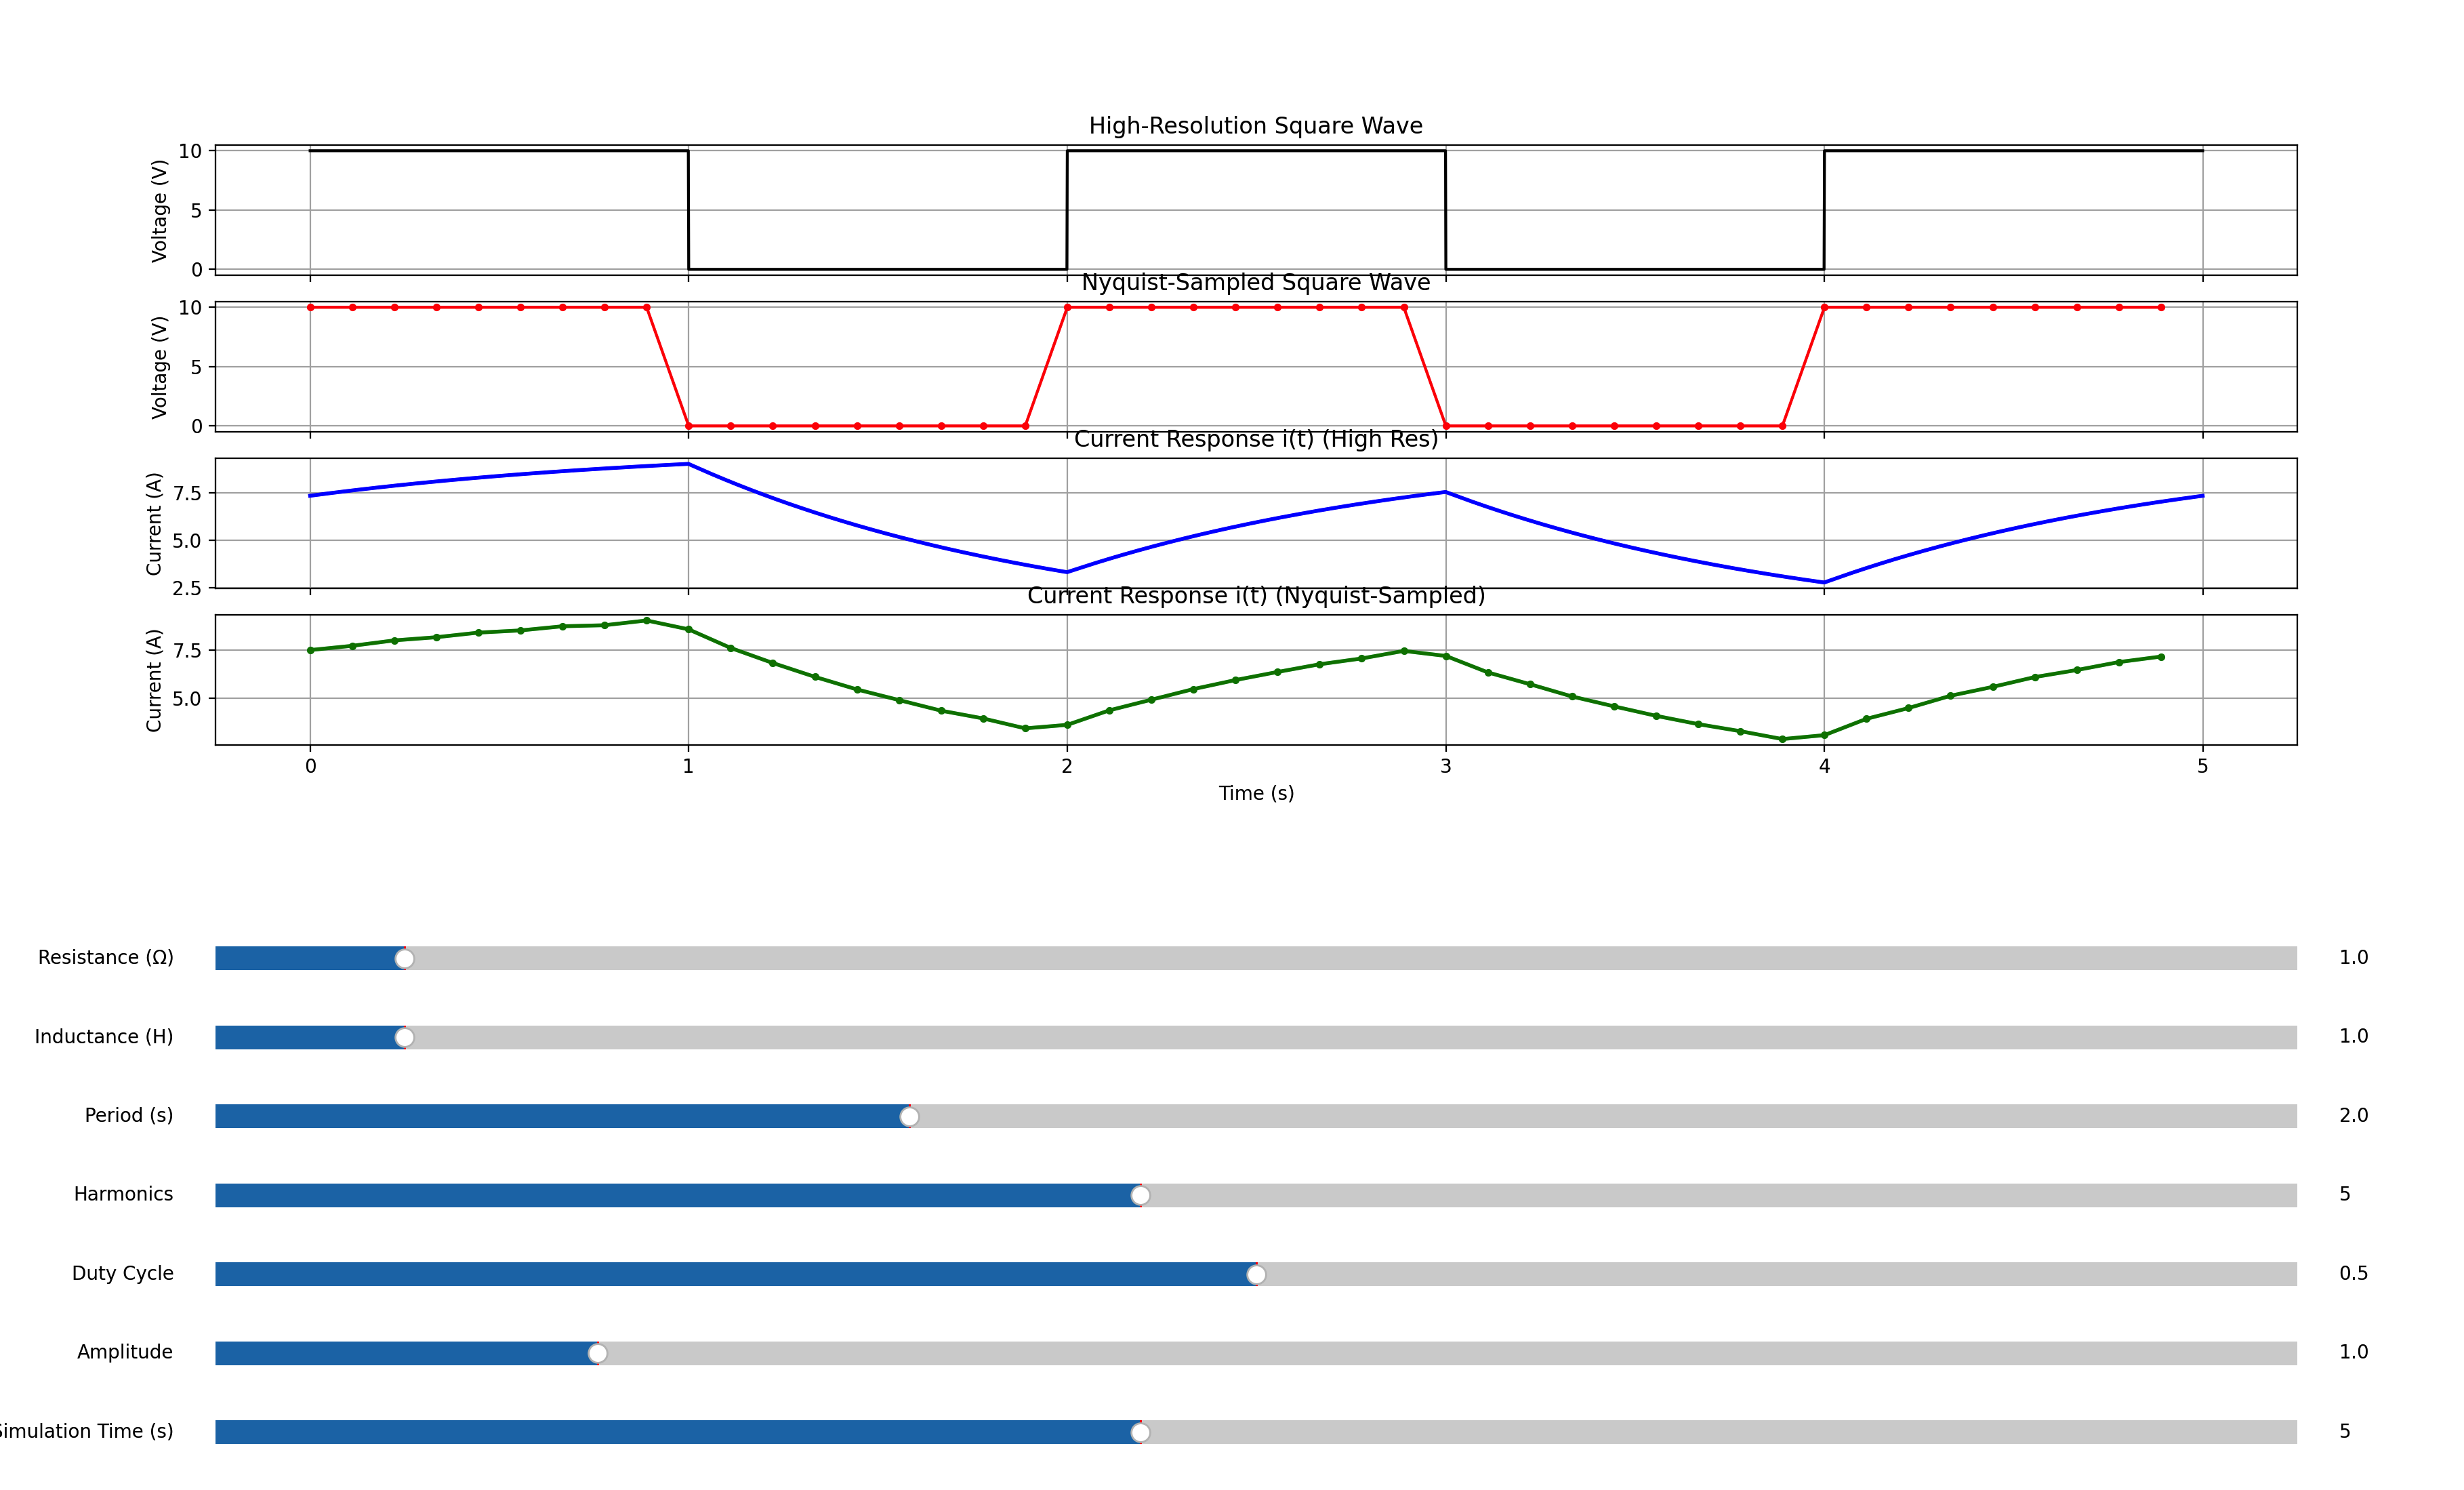
\includegraphics[width=0.6\linewidth]{FFT_response/fft}
    \caption{The Plot of the current response through FFT}
    \label{fig:enter-label}
\end{figure}
\textbf{The Difference in the Time complexity between DFT and FFT }
\begin{figure}[H]
    \centering
    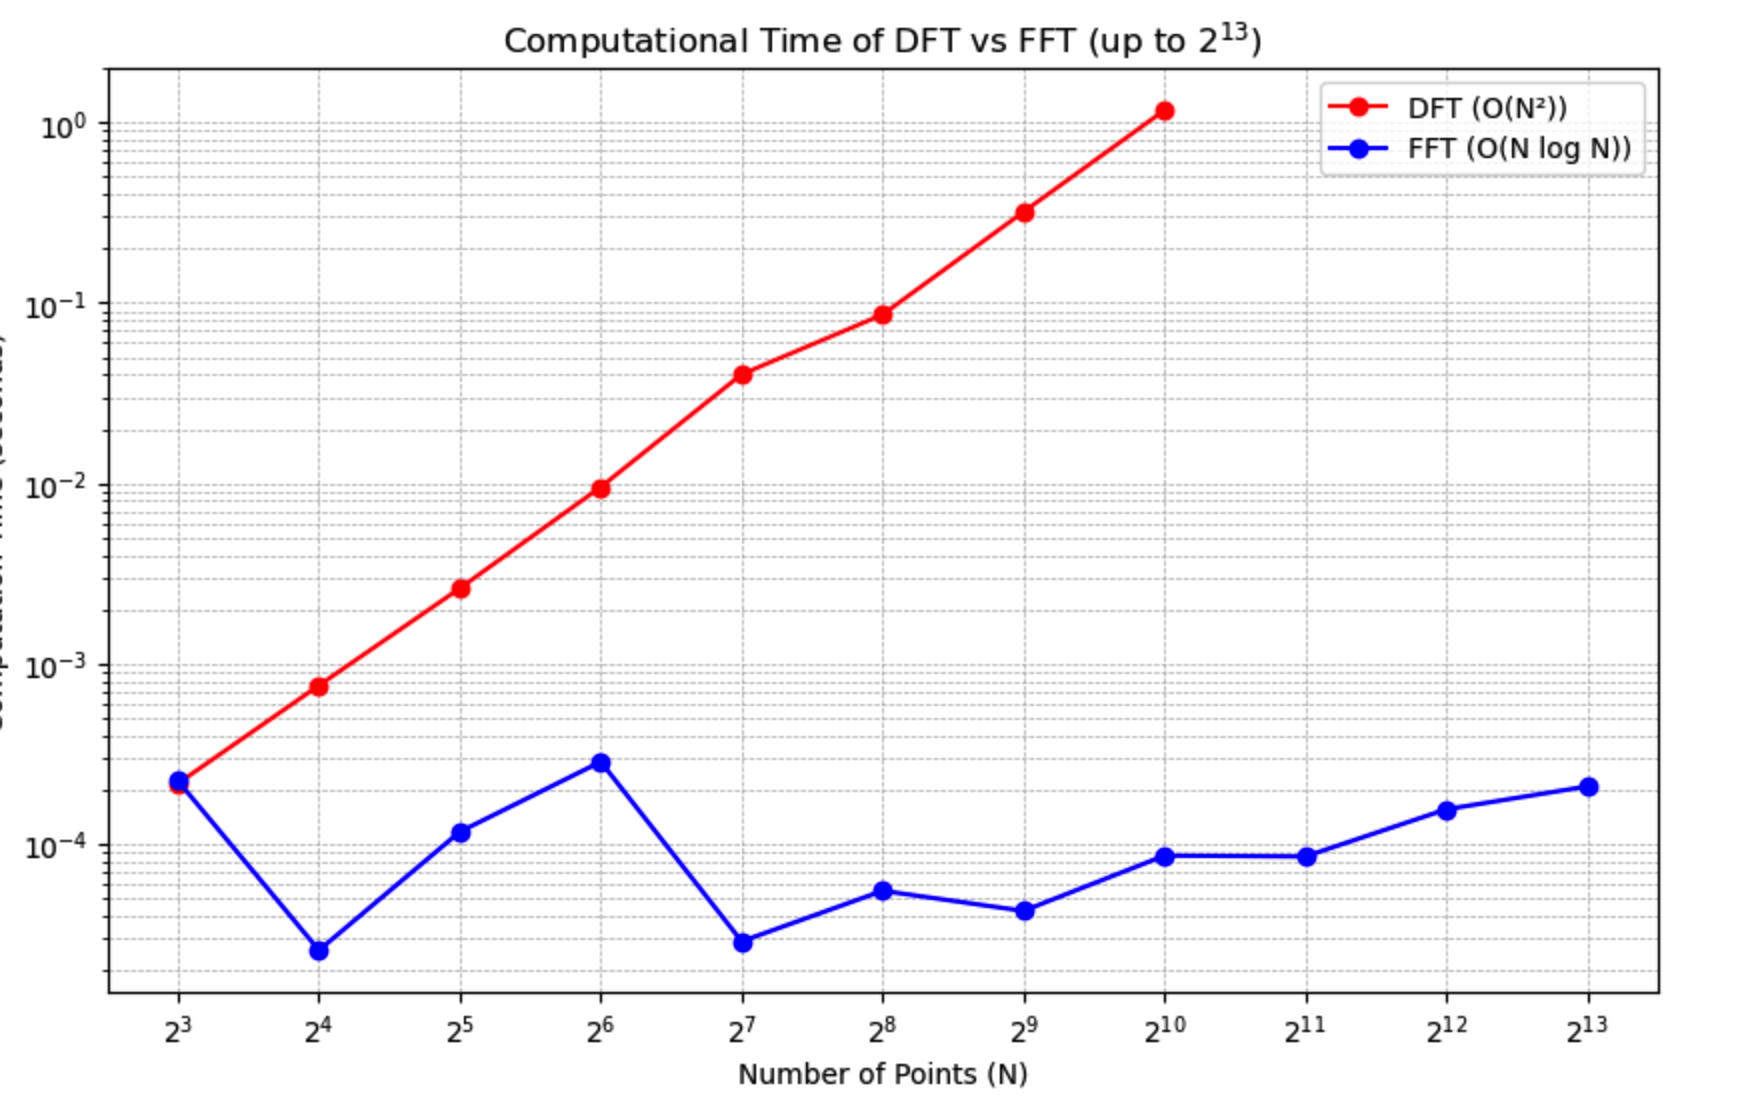
\includegraphics[width=0.6\linewidth]{FFT_response/compare}
    \caption{Difference in the Time complexity between DFT and FFT}
    \label{fig:enter-label}
\end{figure}
\section{Conclution}
We analyzed the response of an RL circuit to a square wave voltage input using the \textbf{Fast Fourier Transform (FFT)}. We demonstrated how the Fourier domain approach simplifies solving the differential equation, allowing us to compute the current response efficiently. Additionally, we explored the impact of \textbf{Nyquist sampling}, highlighting its role in ensuring accurate numerical computations while optimizing computational resources.

\textbf{Key Findings: }
\begin{enumerate}
    \item FFT-Based Solution for RL Circuits:
    \begin{itemize}
        \item The FFT method provides an efficient way to analyze linear circuit responses in the frequency domain.
        \item By applying the inverse FFT, we accurately retrieve the time-domain current response.
    \end{itemize}
    \item Nyquist Sampling and Computational Efficiency:
    \begin{itemize}
        \item Sampling at or above the Nyquist rate preserves essential frequency components while minimizing data redundancy.
        \item Increasing the sampling rate beyond a certain threshold does not significantly alter the output current waveform, confirming the sufficiency of Nyquist's criterion.
    \end{itemize}
    \item Effect of Circuit Parameters:
    \begin{itemize}
        \item The RL circuit acts as a low-pass filter, smoothing the square wave input by attenuating higher harmonics.
        \item he response shape is influenced by the resistance R, inductance L, and the duty cycle of the input square wave.
    \end{itemize}
    \item Practical Implications:
    \begin{itemize}
        \item Understanding sampling limitations is crucial for real-world signal processing and embedded systems applications.
        \item The interactive implementation enables real-time visualization of how different parameters affect the circuit's behavior.

    \end{itemize}
\end{enumerate}
\end{document}
